
\chapter{Introdução}
 
 \section{Motivação e Lacuna}
 \label{sec:Motivacao}
%   A contagem de objetos deu origem aos números que suscetivamente originou os cálculos e conforme a evolução humana acontece técnicas para auxiliar a contagem e cálculos estão cada vez mais acentuada, pois em vários meios para se obter um resultado no mundo real, é necessário ainda mão de obra humana, além de requerer um certo tempo. 

%    A interação com humanoides faz parte do imaginário humano desde os períodos históricos. Através da capacidade computacional de processar dados, viu-se ali a possibilidade de tornar real a simulação da vida biológica em modelos matemáticos. A idealização da inteligência artificial estabeleceu a necessidade da Visão Computacional, área que abrange a habilidade de máquinas visualizarem e reconhecerem o contexto apresentado por imagens. Desde então Redes Neurais Artificiais tem sido aplicadas com o objetivo de detectar e predizer objetos, afim de compreender situações \cite{DBLP:journals/corr/BadrinarayananK15}. As subáreas como Aprendizagem de Máquina e Aprendizagem Profunda compreendem técnicas para detecção de certos padrões com a intenção de predizer itens presentes em figuras \cite{Goodfellow-et-al-2016}.
    
A aprendizagem profunda (\textit{Deep Learning}) tem se destacado no cenário de Visão Computacional e as Redes Neurais Convolucionais (CNN) \cite{Simonyan14c} tem dominado o estado da arte \cite{ANN}. Estudos podem ser encontrados para detecção de objetos \cite{DBLP:journals/corr/abs-1904-00889, 8437104, 8489369, rs11010011, 8186148}, segmentação de imagens \cite{Zhao2017CVPR,DBLP:journals/corr/CaoSWS16}, contagem de objetos \cite{8186148,DBLP:journals/corr/CaoSWS16,articleLuiz}, entre outros.
    
Entre as diversas aplicações da Visão Computacional, os métodos de contagem e localização de objetos consistem em detectar e obter a posição de cada objeto individualmente na imagem.
Esses métodos tem auxiliado no controle e contagem de pessoas \cite{ExtractHuman}, carros \cite{CarCount}, animais \cite{8639306}, e até mesmo bactérias \cite{7320116}.
    A maioria dos métodos de contagem são baseados nos mais conhecidos métodos de detecção de objetos (Faster-RCNN \cite{DBLP:journals/corr/Girshick15}, RetinaNet \cite{DBLP:journals/corr/abs-1708-02002}, YoloV3 \cite{DBLP:journals/corr/abs-1804-02767}).
    Esses métodos consideram um retângulo envolvente para cada objeto e podem fornecer tanto a posição (centro do retângulo envolvente) como a contagem (número de retângulos envolventes). 
    %Layout Proposal Networks (LPNs) \cite{8237708} é um método recente que tem seguido a proposta de detecção de objetos para contagem.
    
    Embora os métodos recentes tenham obtido resultados promissores, três desafios ainda se mantêm.
    O primeiro desafio é a alta densidade com objetos sobrepostos.
    Em geral, os métodos de detecção de objetos não são adequados para cenários densos de objetos \cite{Goldman2019CVPR}.
    Neste caso, a grande sobreposição dos retângulos envolventes devido a oclusão dificulta o aprendizado dos métodos. Layout Proposal Networks (LPNs) \cite{8237708} é um método recente que tem seguido a proposta de detecção de objetos para contagem de carros utilizando camadas da VGG-16. Seu maior problema na contagem está na sobreposição dos retângulos quando carros estão lado a lado na imagem, como em um estacionamento. 
    %Na vida real temos como preceito a idéia de que dois corpos não ocupam o mesmo espaço, as CNN's por sua vez detectam bordas, textura e cor de espaços pré-definidos nos experimentos (rotulação) através das camadas convolucionais nas imagens (\cite{deeplearningbook}).
    
    
    Por outro lado, estimar um mapa de densidade para obter a quantidade de objetos tem apresentado resultados promissores \cite{DBLP:journals/corr/abs-1808-01050,880968,Cao2017} e  feito com que estudos tenham esta direção.
    Um mapa de densidade consiste em estimar a probabilidade de um objeto ocorrer em cada pixel da imagem.
    Porém a diversidade encontrada nos cenários das imagens (e.g., escala, rotação, etc) dificulta a detecção e contagem por um mapa de densidade. Assim alguns trabalhos buscam encontrar um método eficaz que faça com que o objeto de interesse tenha um destaque nas probabilidades estimadas \cite{inproceedings} \cite{DBLP:journals/corr/abs-1711-04433}.
    
    O segundo desafio é a necessidade da rotulação detalhada das imagens, o que é difícil de obter em grandes quantidades. 
    A rotulação de um retângulo envolvente para cada objeto na imagem torna-se inviável para cenas muito densas em grandes quantidades de imagens.
     Por outro lado, a utilização de um único ponto para rotular cada objeto \cite{8237708} tem sido grande alvo de estudos.
     Por exemplo, \cite{DBLP:peri/corr/abs-1904-01333} propõem o método de detecção e contagem de multidões usando pontos na cabeça das pessoas. 
     Os métodos baseados apenas em pontos consideram a informação de contexto ao redor do ponto, pois os objetos compartilham cores, textura e forma.
     Dessa forma, os métodos tendem a reconhecer mesmo que os limites dos objetos não estejam delimitados durante o aprendizado \cite{Aich2018ImprovingOC}.

    O terceiro desafio consiste em contar e localizar objetos em uma sequência de imagens.
   A análise do movimento que objetos realizam nos vídeos podem fornecer informações valiosas que nem sempre são consideradas na contagem de objetos em uma imagem.
Nesse contexto, alguns pesquisadores demonstram em seus estudos que rastrear o movimento pode auxiliar na detecção e reconhecimento, assim como distingui-los do fundo (\cite{Ma_2015_ICCV,Nam_2016_CVPR,Danelljan_2015_ICCV_Workshops,WANG201962,8898173,ExtractHuman}).  
   Diferente do rastreamento de objetos, o objetivo deste trabalho é considerar as informações do passado para contar e localizar os objetos em um quadro atual.
    
    Para contornar os desafios citados acima, este trabalho propõe um método para localizar e contar objetos em vídeos usando redes neurais convolucionais.
    %Dada uma imagem de entrada
    Dado um quadro de um video e o quadro anterior, o método proposto estima uma mapa de densidade com a probabilidade de ocorrência de um objeto em cada pixel.
    Dessa forma, a rotulação apenas de pontos é suficiente para o treinamento do método e cenas densas podem ser melhor modeladas.
    %o método proposto considera as predições das posições dos objetos no quadro anterior.
    Além disso, o método proposto também estima um mapa de vetores de deslocamento, isto é, vetores que indicam a direção do movimento de cada pixel da imagem.
    Essa estimativa dos vetores de deslocamento também é usada para predizer o mapa de densidade de um quadro atual.
    Todas essa informações são concatenadas para estimar a localização e contagem de objetos do quadro atual.
    Resultados experimentais mostram que a concatenação dessas informações é capaz de melhorar a contagem e localização dos objetos.
    
    
    
    %Pontos estratégicos na posição de cada objeto é usado como rotulagem. A hipótese aposta nas posições por onde o objeto percorreu anteriormente para estimar o ponto onde ele pode ser encontrado.
    %O método é dividido em quatro fases principais: 1) geração do mapas de recurso usando a VGG19 para cada quadro processado; 2) refinamento do mapa de recursos usando as localizações anteriores; 3) estágios múltiplos de refinamento dos mapas de confiança combinados com o mapa obtido das posições anteriores; e 4) a obtenção da posição do objeto através de picos no mapa de confiança. Os parâmetros foram avaliados na contagem de alevinos presentes no conjunto de dados.


%    A contagem de peixes está entre um dos desafios a serem solucionados para se obter uma solução automática e rápida.
   
%   A pesca está presente no dia-a-dia de milhões de pessoas pelo mundo e pondera fortemente a alimentação, cultura e economia. Por ser o combustível de vários povos na história, se tornou fundamental na alimentação nos períodos modernos. Apesar de muitos grupos ainda utilizarem o peixe como fonte única de nutrição, a sua comercialização move uma porcentagem significativa da economia em vários países singulares na criação e exportação. A China, por exemplo, possui uma participação acima de 60\% da produção mundial de peixe \cite{OECD}\cite{FAO}.
   
%   A produção brasileira de peixes tem crescido nos últimos anos \cite{FAO}. Estima-se que o país latino-americano por possuir um clima favorável e recursos hídricos, possa ter um aumento de 104\% na produção pesqueira até o ano de 2025. Em 2018 a produção teve um crescimento de 4,5 toneladas\cite{EMBRAPA}. 

%   O estado de Mato Grosso do Sul-MS ocupa o 10º lugar na lista dos maiores produtores de peixes de cultivo do Brasil com 25.850 toneladas produzidas. O primeiro lugar vem sendo ocupado nos últimos anos pelo Paraná com 129.900 toneladas \cite{PeixeBR,OECD}.
   
%  O cultivo de peixes sofre grandes intervenções de mercado, com o objetivo de manter a segurança alimentar e ambiental \cite{Aqua}.
%  No sentido de corresponder a demanda mercantil, determinadas espécies necessitam de adaptações, para um clima específico e até mesmo alterações na alimentação.
%  Assim organizações de aquicultura (piscicultura) buscam opções tecnológicas para um máximo aproveito do produto comercializado.
  
%O foco principal desta dissertação está em 
  
  
  % produção de peixe continuará a aumentar para quase 200 Mt em 2026.

\section{Aplicação em Contagem de Peixes}
\label{sec:Aplicação}

%Aplicar técnicas de Aprendizado Profundo para automatizar a contagem de objetos presente em vídeos utilizando a análise do deslocamento de tais objetos no(s) quadro(s) anterior(es). Contudo, apresentar resultados que comprove tal hipótese utilizando vídeos do mundo real. Para realizar este feito os experimentos foram realizados com vídeos onde contém alevinos. 

O método proposto será aplicado na contagem de peixes e alevinos. Na maioria dos casos, a contagem é um trabalho árduo e requer mão de obra humana atenta, além de ser suscetível a erros.
Por serem sensíveis, os peixes requerem uma afabilidade no manuseio durante a contagem.
Em geral, a contagem acontece por técnicas de barragens \cite{Erikson}, alguns cultivadores realizam a peneiragem para extrair os peixes da água e, dessa maneira, obtêm-se uma estimativa da quantidade de peixes que residem em uma determinada região \cite{OECD,FAO}.


A escada de peixes é uma das maneiras utilizadas na contagem.
Assim os peixes passam por barragens conforme a Figura \ref{fig:escadadepeixes} (a). Na usina hidrelétrica de Igarapava do rio Grande \cite{UHE}, pesquisadores construíram salas (Figura \ref{fig:escadadepeixes} (b)) abaixo do nível d'água, sendo possível enxergar os peixes conforme eles atravessam.
Especialistas na área buscam encontrar técnicas para automatizar a contagem dos peixes que transitam a hidrelétrica.


\begin{figure}[!ht]
	\centering
		\subfloat[]{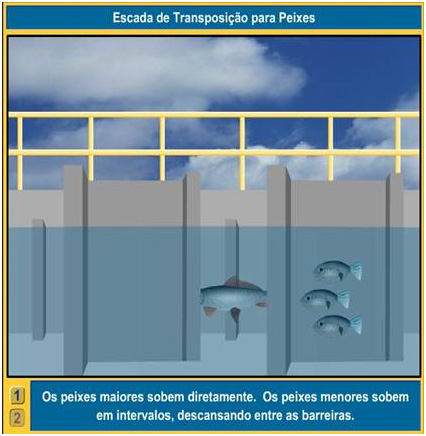
\includegraphics[width=0.4\textwidth]{image/escadadepeixes.jpg}}\vspace{0.3cm}
	    \subfloat[]{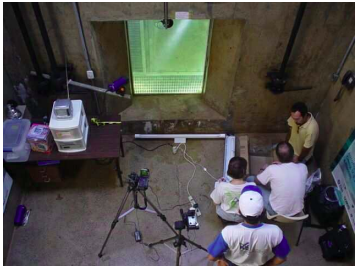
\includegraphics[width=0.55\textwidth]{image/saladaagua.png}}
	\caption{(a) Ilustração da Escada de peixes - \cite{UHE}, (b) sala abaixo do nível d'água \cite{Erikson}.}
	\label{fig:escadadepeixes}
\end{figure}

Os cultivadores precisam ter o controle da quantidade de peixes vivos presentes em seus cativeiros, para que a alimentação seja devidamente proporcional para todos, e se há necessidade do cultivo de novos peixes, ou até mesmo alterações no meio. É notória a necessidade de uma exatidão da quantidade que residem uma região. 


\section{Objetivos}
\label{sec:objetivos}

\section{Objetivo Geral}
O objetivo deste trabalho é propor um método para contagem de objetos em vídeos utilizando redes neurais convolucionais.
Um dos intentos principais está em detectar tais objetos nas imagens levando em consideração a posição espacial no quadro anterior. Assim com a ciência das localizações anteriormente, uma estimativa mais refinada da posição atual pode ser obtida.

%Os peixes presentes no \textit{dataset} utilizado se locomovem irrefletidamente e como foram recém chocados, possuem um tamanho muito reduzido quando comparado a fase adulta. Assim os alvos a serem alcançados está em analisar parâmetros que se adaptam a esses peixes de maneira que a contagem seja a mais exata possível.

\section{Objetivos Específicos}

%O foco dos experimentos pode ser descrito como uma análise dos parâmetros para aperfeiçoar a técnica proposta, de modo que se ajuste adequadamente ao conjunto de dados. 
%Os peixes presentes no \textit{dataset} utilizado se locomovem irrefletidamente e como foram recém chocados, possuem um tamanho muito reduzido quando comparado a fase adulta. Assim os alvos a serem alcançados está em analisar parâmetros que se adaptam a esses peixes de maneira que a contagem seja a mais exata possível.

Tendo o objetivo geral imposto, os seguintes objetivos específicos foram definidos:
%
\begin{enumerate}
    %\item Gerar um volume de entrada, contendo a imagem de entrada e os vetores de deslocamento dos objetos no quadro anterior.
    \item Estimar a contagem por meio de um mapa de densidade obtido por uma rede neural convolucional;
    \item Avaliar a inclusão do quadro anterior na estimativa do quadro atual;
    \item Incluir vetores de deslocamento na predição do mapa de densidade;
    \item Aplicar o método na contagem de alevinos.

\end{enumerate}

%Para alcançar os objetivos específicos foram realizadas as seguintes atividades:

%\begin{enumerate}
    %\item Rotular cada peixe presente nos quadros de maneira que os pontos represente cada alevino;
    %\item Gerar o \textit{Ground Truth} com base nos pontos para os quadros atuais e o um vetor de deslocamento para cada peixe;
    %\item Gerar o mapa de recursos para os quadros processados com a VGG19, depurar os mapas resultantes com estágios de refinamento.
    %\item Gerar o mapa de recursos do(s) quadro(s) anterior(es) dos quadros atuais processados com a VGG19, depurar os mapas resultantes com estágios de refinamento.
   % \item Concatenar os mapas dos quadros anteriores e atuais conforme os estágios são aplicados;
  %  \item Treinar a CNN proposta com vários parâmetros para o ajuste ao conjunto de dados;
 %   \item Estimar um linear para detectar os picos nos mapas de densidades resultantes do modelo treinado;
%    \item Testar e avaliar os resultados qualitativamente e quantitativamente;
%\end{enumerate}


%\section{Principais Contribuições}
%\label{sec:contribuicoes}


%\section{Organização}
%\label{sec:organizacao}


